%*****************************************
\chapter{Simulation}\label{ch:simulation}
%*****************************************
\section{The Robot}\label{sec:nuga}
Nuga is Paltech's solution for speeding up the weed removal process. Nuga is a mobile platform equipped with two drilling mechanisms, also called \ac{IT}, one main camera at the front for plant detection, two internal cameras for fine adjustment during tools' placement, an IMU, and two GNSS antennas for GPS localization. Each \ac{IT} is mounted on a structure with three \ac{DOF} using prismatic joints, allowing movement in X, Y, and Z directions.

\begin{figure}[bth]
    \centering
    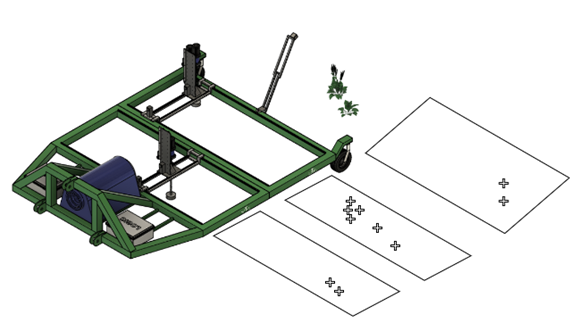
\includegraphics[width=0.7\linewidth]{gfx/ch02/nuga_cad.png}
    \caption{Nuga Platform}
    \label{fig:nuga-cad}
\end{figure}


% See classicthesis-config.tex for changing the prefixes of the refs
% Testing for autoref: \autoref{ch:intro}, \autoref{ch:examples}, and \autoref{sec:new}

%Testing for ``clever'' references: \cref{ch:intro} and \cref{ch:examples}
% Ugly work-around
% Part~\textsc{\ref{pt:showcase}}


\section{Simulation}\label{sec:simulation}
A representative simulation of reality is crucial for developing new algorithms and analyzing robot behavior before real-world implementation. Therefore, building a simulation of the project was a foundational step for this work, ensuring a controlled environment for validation and testing. Gazebo\footnote{Gazebo is a physics-based robotics simulation tool that allows testing and validation of robot models before real-world deployment. \url{https://gazebosim.org/home}} was the selected tool because it provides a physics engine, supports sensor and actuator modeling, and integrates well with ROS\footnote{ROS (Robot Operating System) is an open-source framework that provides tools, libraries, and conventions for developing, managing, and simulating robotic applications. \url{https://www.ros.org/}}, making it ideal for testing robotic systems.

The simulation consists of six key components: URDF files define the robot's structure and properties, SDF files describe the virtual environment, and Gazebo plugins provide additional functionality, such as simulating custom sensors, actuators, or control interfaces. Additionally, core system operations include joint control for managing the movement of the \ac{IT}, localization for tracking the robot’s position, and weed detection, which relies on an AI model for Rumex recognition. \autoref{fig:building-sim} illustrates these components as building blocks for the simulation.

\begin{figure}
    \centering
    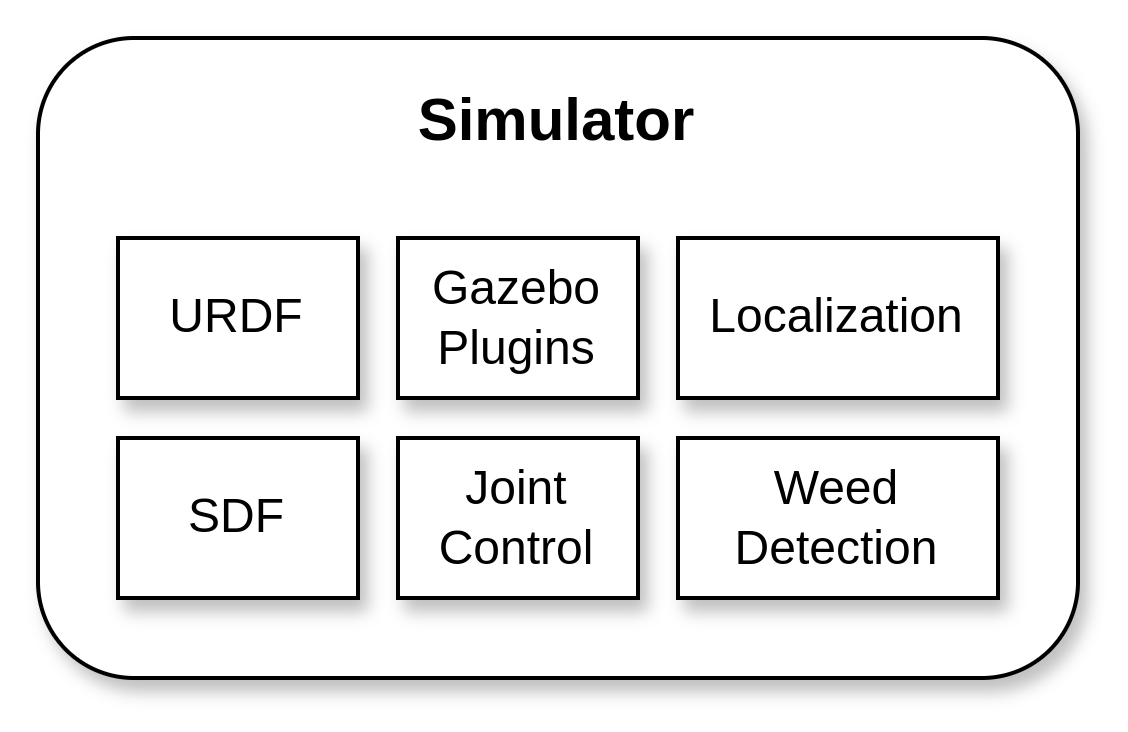
\includegraphics[width=0.5\linewidth]{gfx/ch02/simulator.png}
    \caption{Simulator Components}
    \label{fig:building-sim}
\end{figure}

\subsection{URDF}
\ac{URDF} is an XML file used to describe multibody systems for robot simulation. It defines the visual, collision, and inertial properties of rigid body objects, as well as their connections (\emph{joints}). This establishes a spatial relationship between frames, which ROS and Gazebo can later interpret for control and visualization. This file also allows modeling different types of sensors and incorporating Gazebo plugins to link it with ROS control actions. We exploit these capabilities to define camera intrinsics, IMU behavior, GPS properties, and control the \ac{IT} using \texttt{ros2\_control}\footnote{\texttt{ros2\_control} is a ROS 2 framework that provides a standardized interface for managing hardware, enabling modular and reusable control systems for robots. \url{https://control.ros.org/rolling/doc/getting_started/getting_started.html}}.

\autoref{fig:urdf-structure} displays the structure of the URDF files, being nuga the highest level entity that joins the robot description, gazebo sensor modeling and plugins, as well as \texttt{ros2\_control} configuration. Nuga description defines the robot's physical structure, including its links (e.g., chassis, wheels, camera support), joints (fixed, continuous, prismatic connections), sensors (cameras, IMU, GPS), and inertial properties. It organizes these components into a kinematic tree (e.g., base\_link -> chassis\_link -> wheels/sensors) using macros for modularity, and resulting in the model displayed in \autoref{fig:nuga-urdf}.

\begin{figure}[hbt]
    \myfloatalign
    \subfloat[URDF files structure.]
    {\label{fig:urdf-structure}
        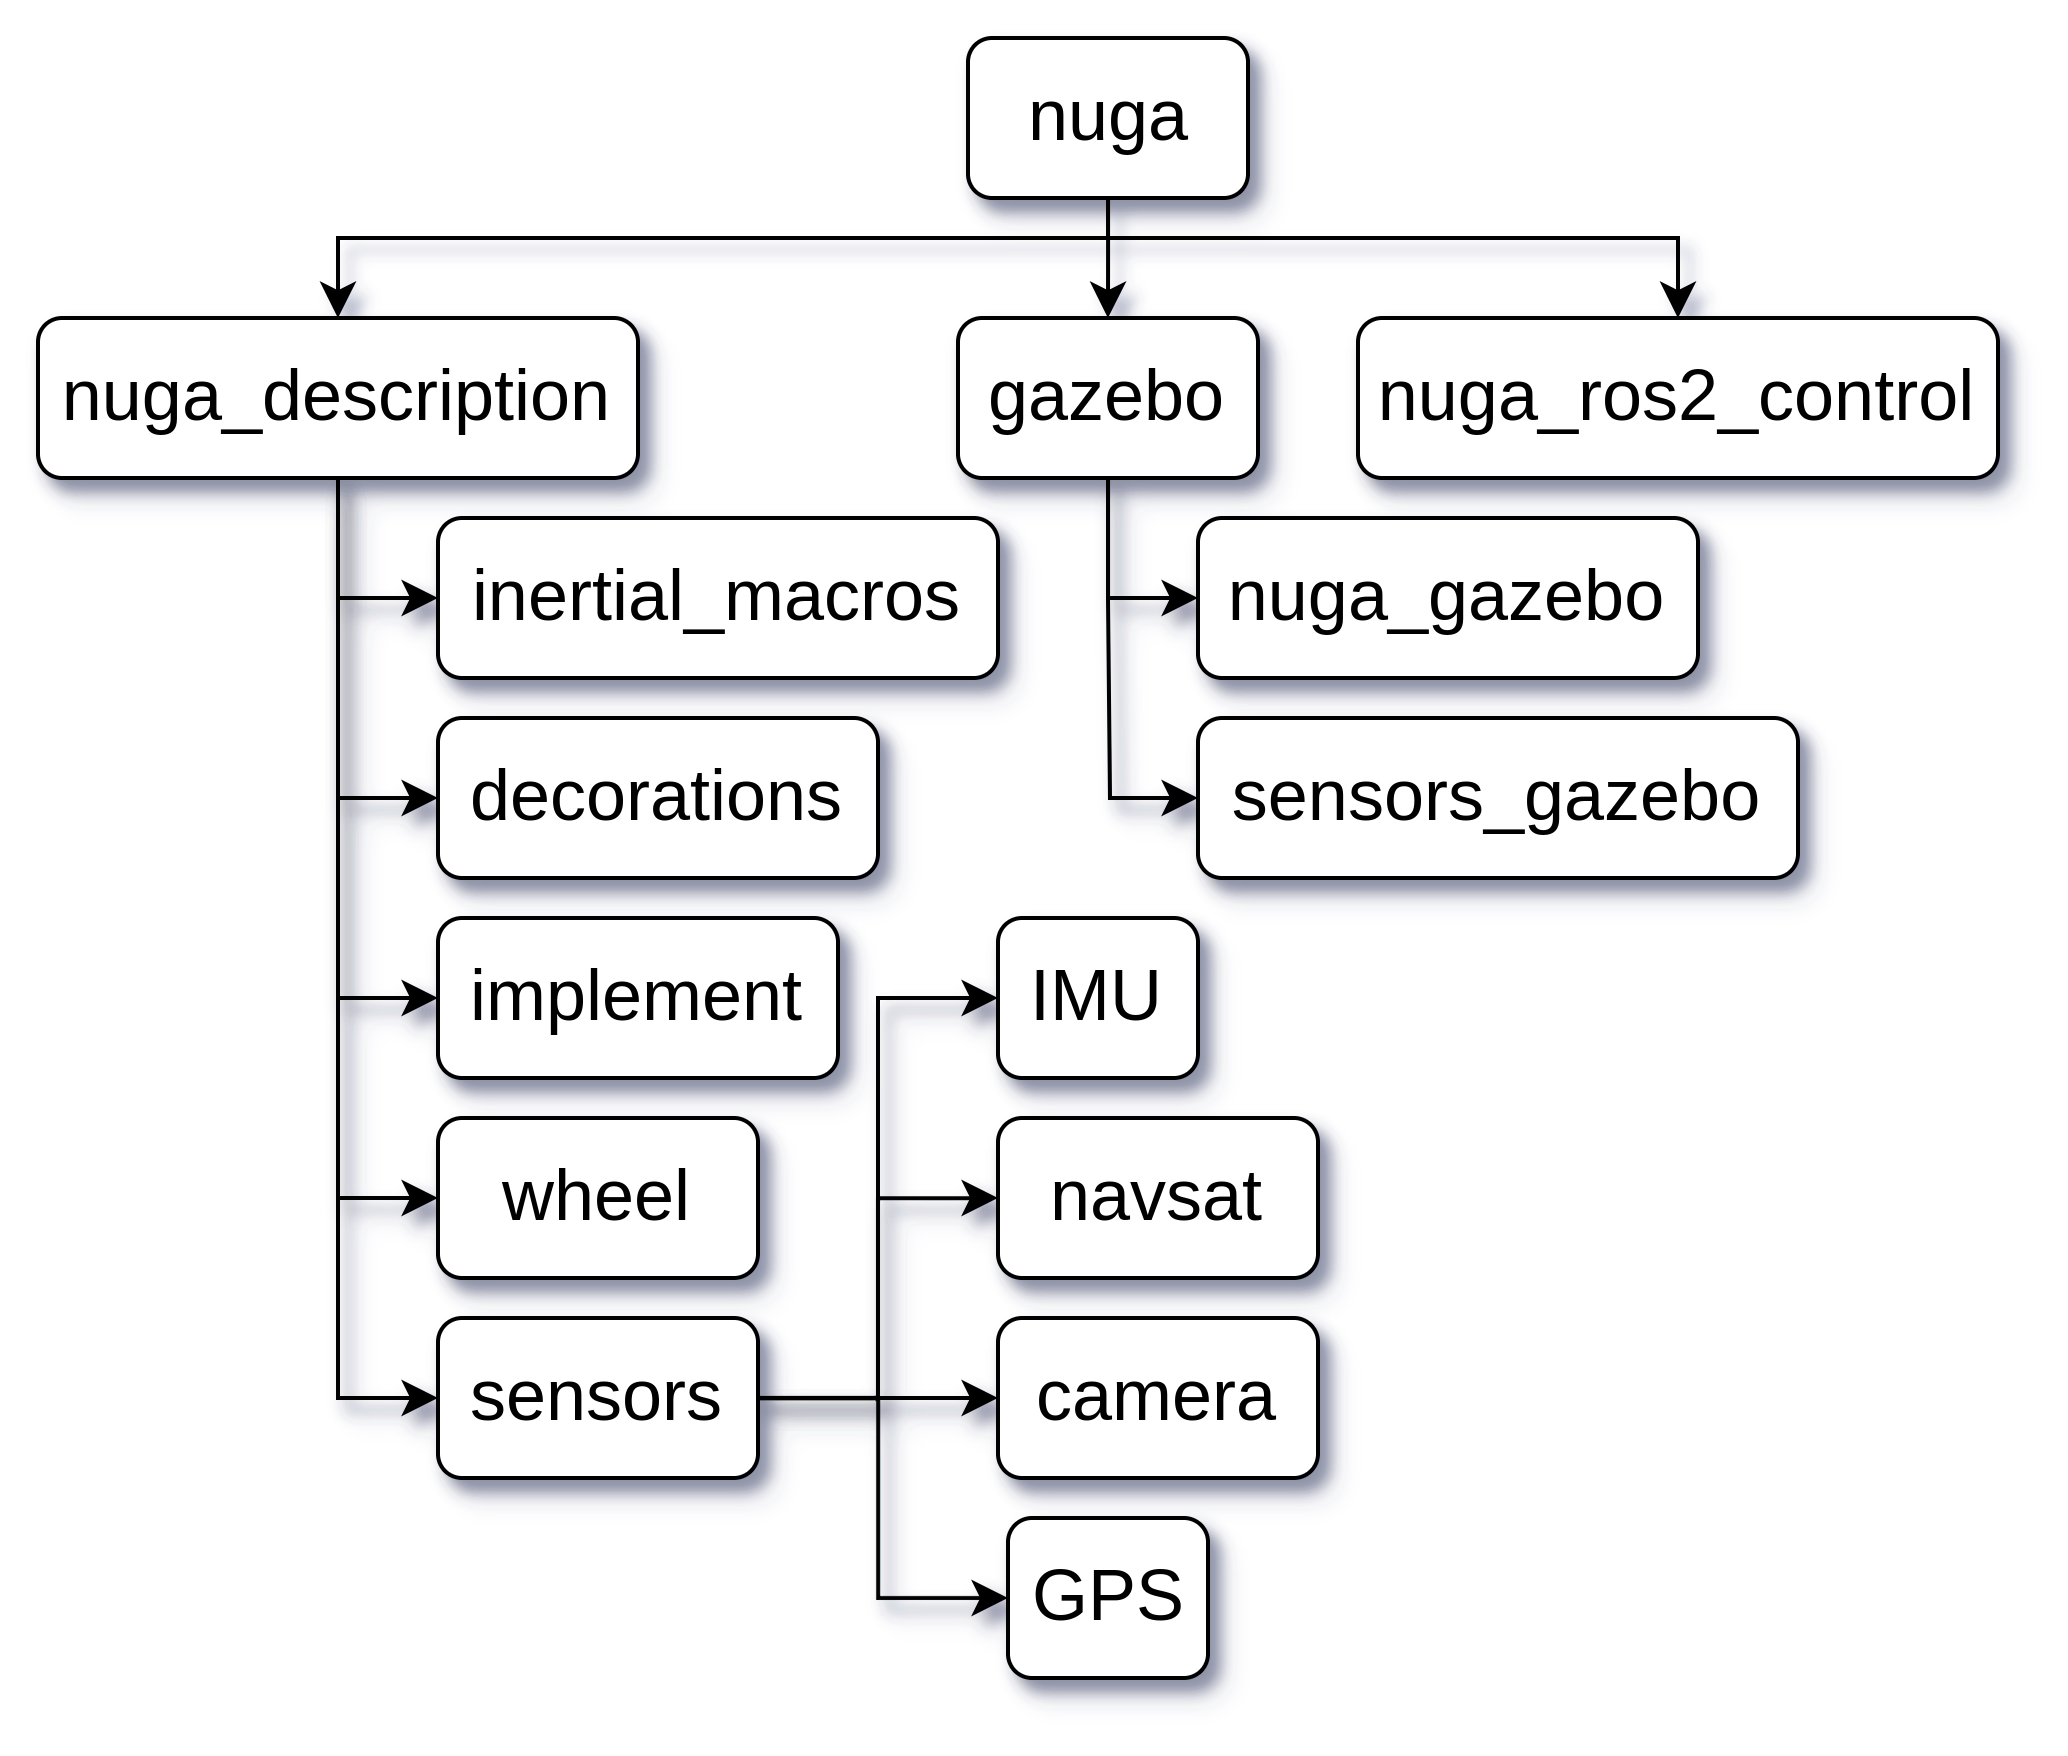
\includegraphics[width=.45\linewidth]{gfx/ch02/urdf.png}} \quad
    \subfloat[RViz visualization of Nuga description.]
    {\label{fig:nuga-urdf}%
        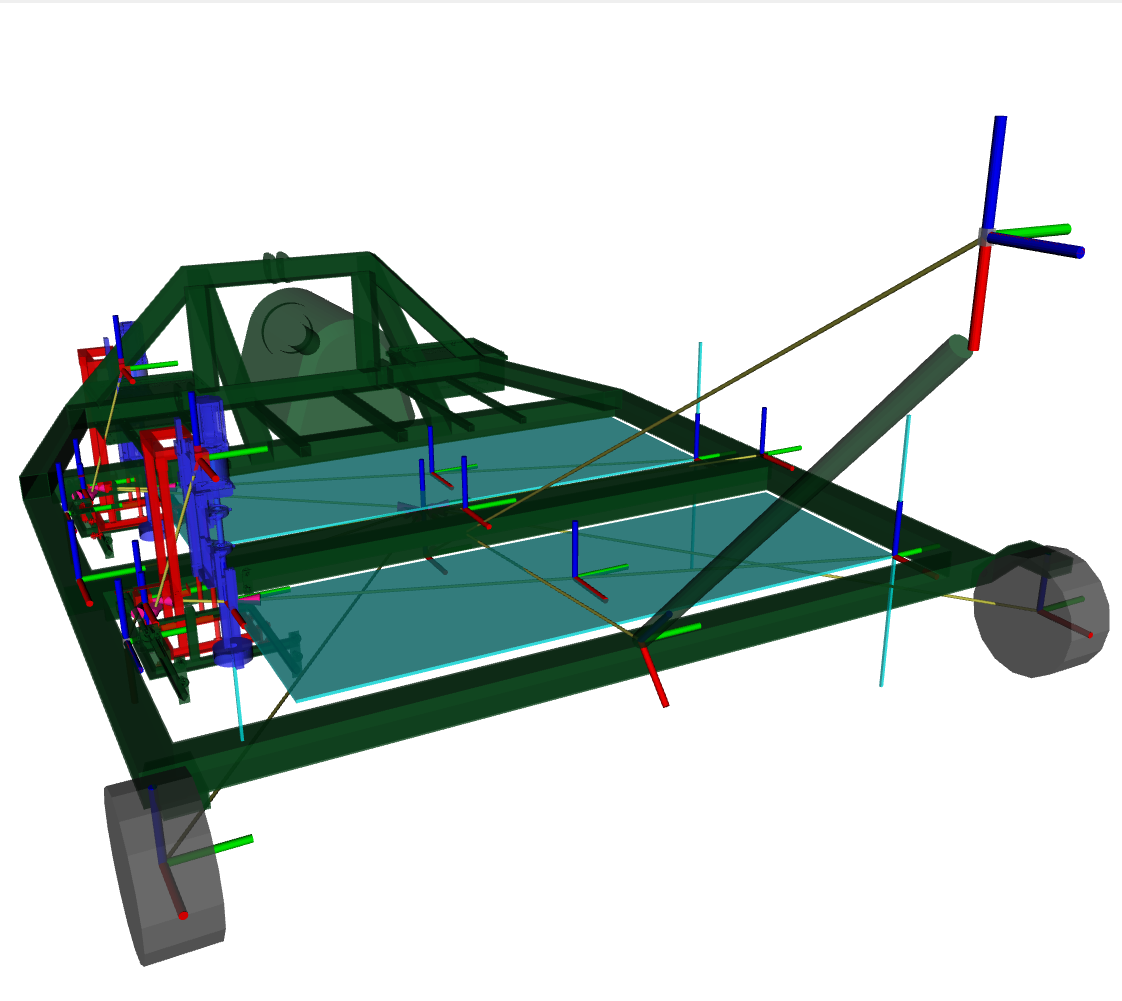
\includegraphics[width=.45\linewidth]{gfx/ch02/nuga_urdf.png}} \\
    \caption[Robot definition using URDF]{Robot definition using URDF}
\end{figure}

\subsection{SDF}
\ac{SDF} also written in XML, describes the properties of the virtual world. Gazebo uses this file to define the terrain, obstacles, lighting conditions, physics parameters, and other environmental elements that affect the robot’s interaction with the simulation. Having repeatability in a simulated world is important for debuging and testing purposes, for this reason a Python script was used to generate easy to configure worlds from a YAML configuration file. An example of the config file is shown in \autoref{lst:world-yaml}. For reproducibility, a seed value is configured in the simulation settings, the weed infestation pattern is defined within quadrants of specified dimensions (\texttt{quadrant\_size}) and each quadrant is individually configured with:

\begin{itemize}
    \item Spatial distribution:
    \begin{itemize}
        \item \textit{uniform}: Random uniform distribution
        \item \textit{clustered}: Random normal distribution with definable standard deviations ($\sigma_x, \sigma_y$)
    \end{itemize}
    \item Weed density: Weeds per square meter (weeds/m²)
    \item Direction: Propagation axis for adjacent quadrants ($\pm x,\pm y$)
    \item Workspace expansion: If \texttt{outside\_workspace} is true, the infestation area extends 10\% beyond the quadrant boundaries.
\end{itemize}

A visual result of the generated world using such configuration file is shown in \autoref{fig:world}.

\begin{figure}[h]
    \centering
    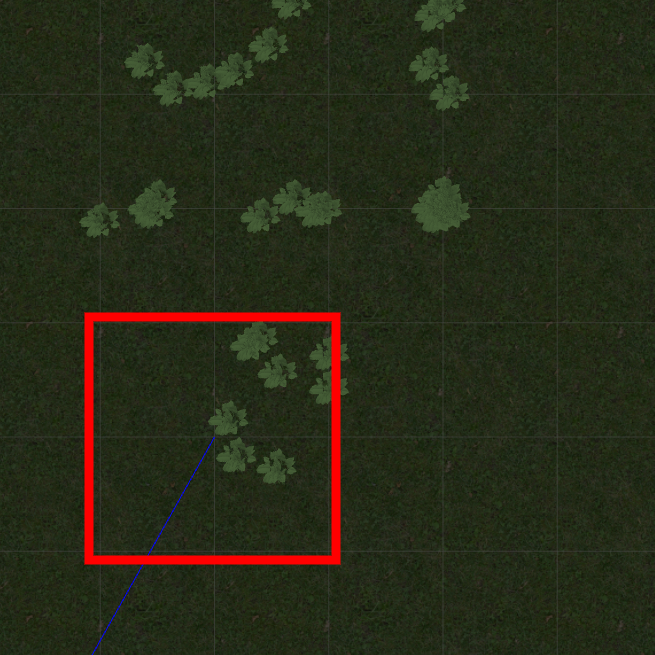
\includegraphics[width=0.4\linewidth]{gfx/ch02/world.png}
    \caption{Weed Infestation Example}
    \label{fig:world}
\end{figure}

\subsection{Gazebo Plugins}
The files \texttt{nuga\_gazebo} and \texttt{sensors\_gazebo} from \autoref{fig:urdf-structure} instantiate and configure Gazebo plugins to define sensor behavior, including optical properties for the camera, as well as update rates and noise models for the IMU and GPS. The file \texttt{nuga\_ros2\_control} on the other hand, establishes an interface between the \ac{IT} 's joints and \texttt{ros2\_control} framework, specifying the command interface (position), controller type (forward position controller), and movement limits, enabling 3-\ac{DOF} prismatic motion for each tool. Regarding movement control of the Nuga vehicle, the \texttt{ros\_planar\_move} plugin satisfied all control requirements given the platform's kinematic constraints, eliminating the need for additional configuration.

\subsection{Joint Control}
The control of both \ac{IT} units was handled using the \texttt{ros2\_control} framework (configuration example shown in \autoref{lst:ros2_control-yaml}), as previously described. This framework provides a seamless transition between simulation and real hardware control. In this context, the \texttt{forward\_command\_controller} was used, which is recommended for simulation because it bypasses PID computations by directly sending commands to simulated joints. These joints already track positions perfectly, without the disturbances or error correction needed in real-world scenarios. Simulators like Gazebo inherently handle ideal position tracking, making closed-loop control redundant. However, when switching to real hardware, replacing it with a \texttt{position\_controller} is needed but straightforward thanks to the flexibility of the framework.

Nuga's workspace layout and dimensions are shown in \autoref{fig:ws}. The gantry carrying the \ac{IT} operates within a zone of $2.09$ m in the $Y$ direction, $0.72$ m in $X$, and $0.26$ m in $Z$. An extraction cycle begins with the gantry moving in $X$ and $Y$ to position the tool above the plant, followed by a downward movement in $Z$ to lower the drill and perform the extraction. The gantry has a maximum speed of $1\frac{m}{s}$ in the $XY$ plane, and each extraction can take up to $45$ seconds per plant. 

\begin{figure}[t]
    \myfloatalign
    \subfloat[$X,Y$ Workspace]
    {\label{fig:xy-ws}
        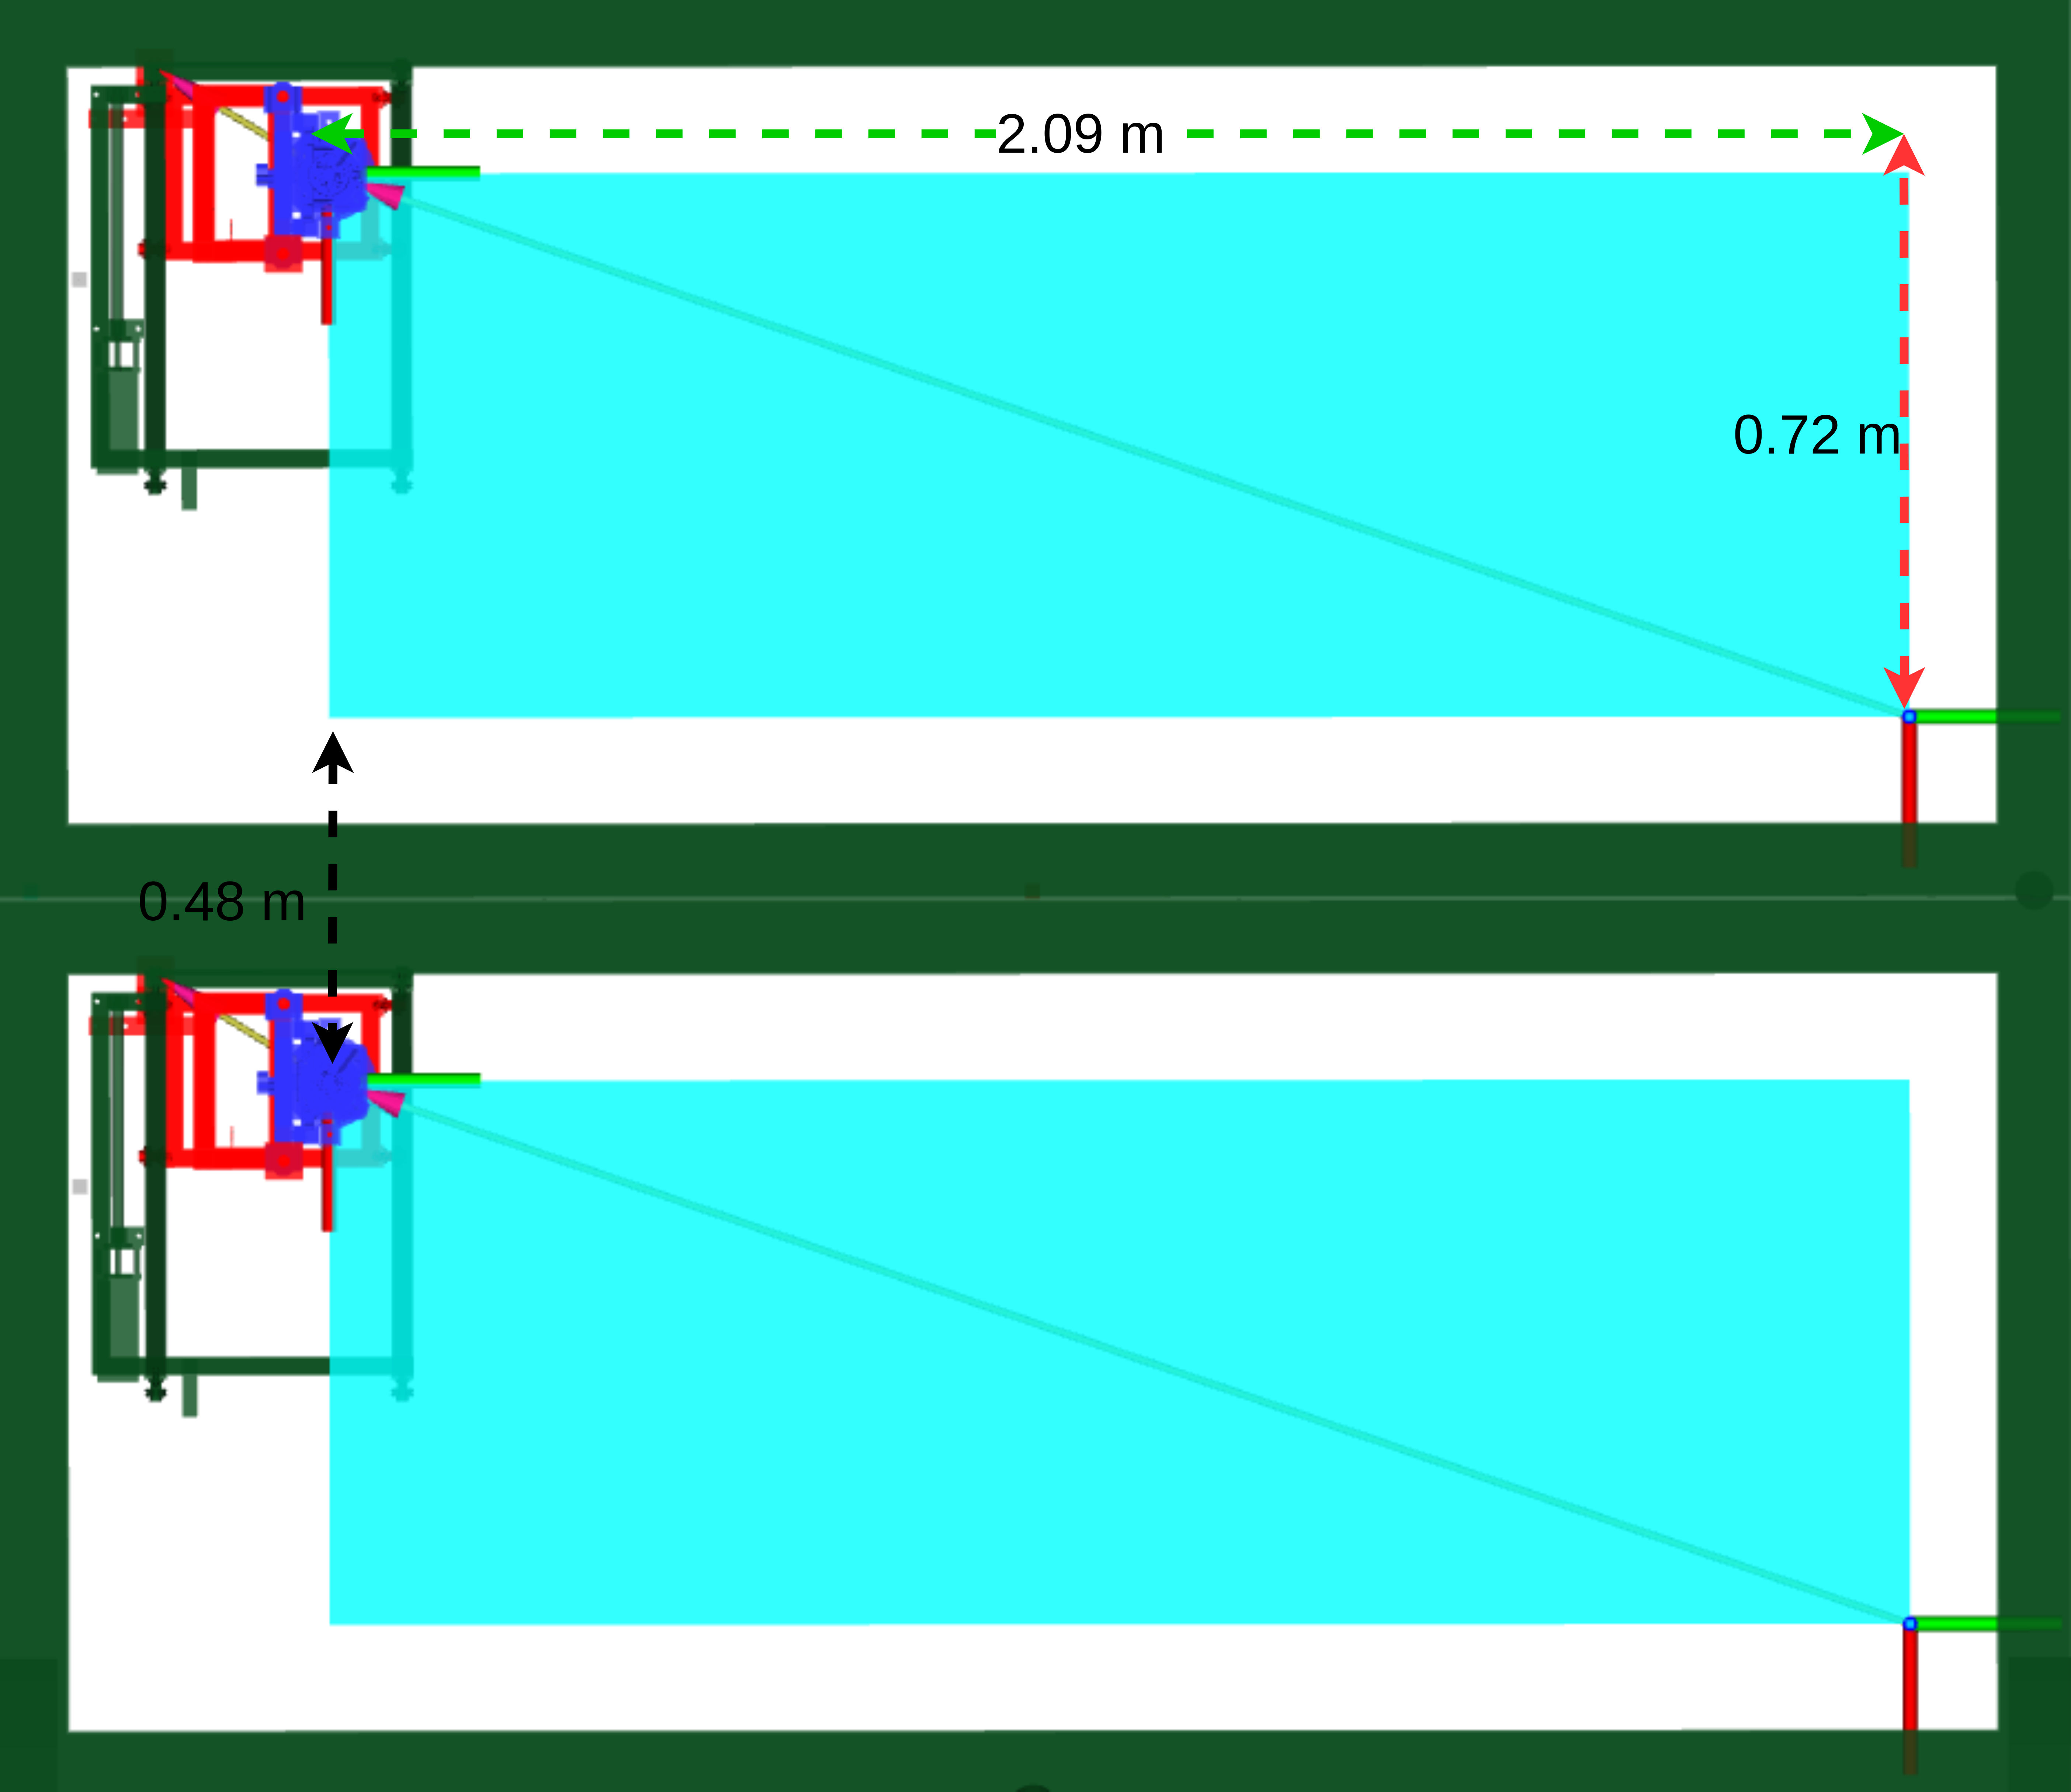
\includegraphics[width=.45\linewidth]{gfx/ch02/xy_ws.png}} \quad
    \subfloat[$Z$ Workspace]
    {\label{fig:z-ws}%
        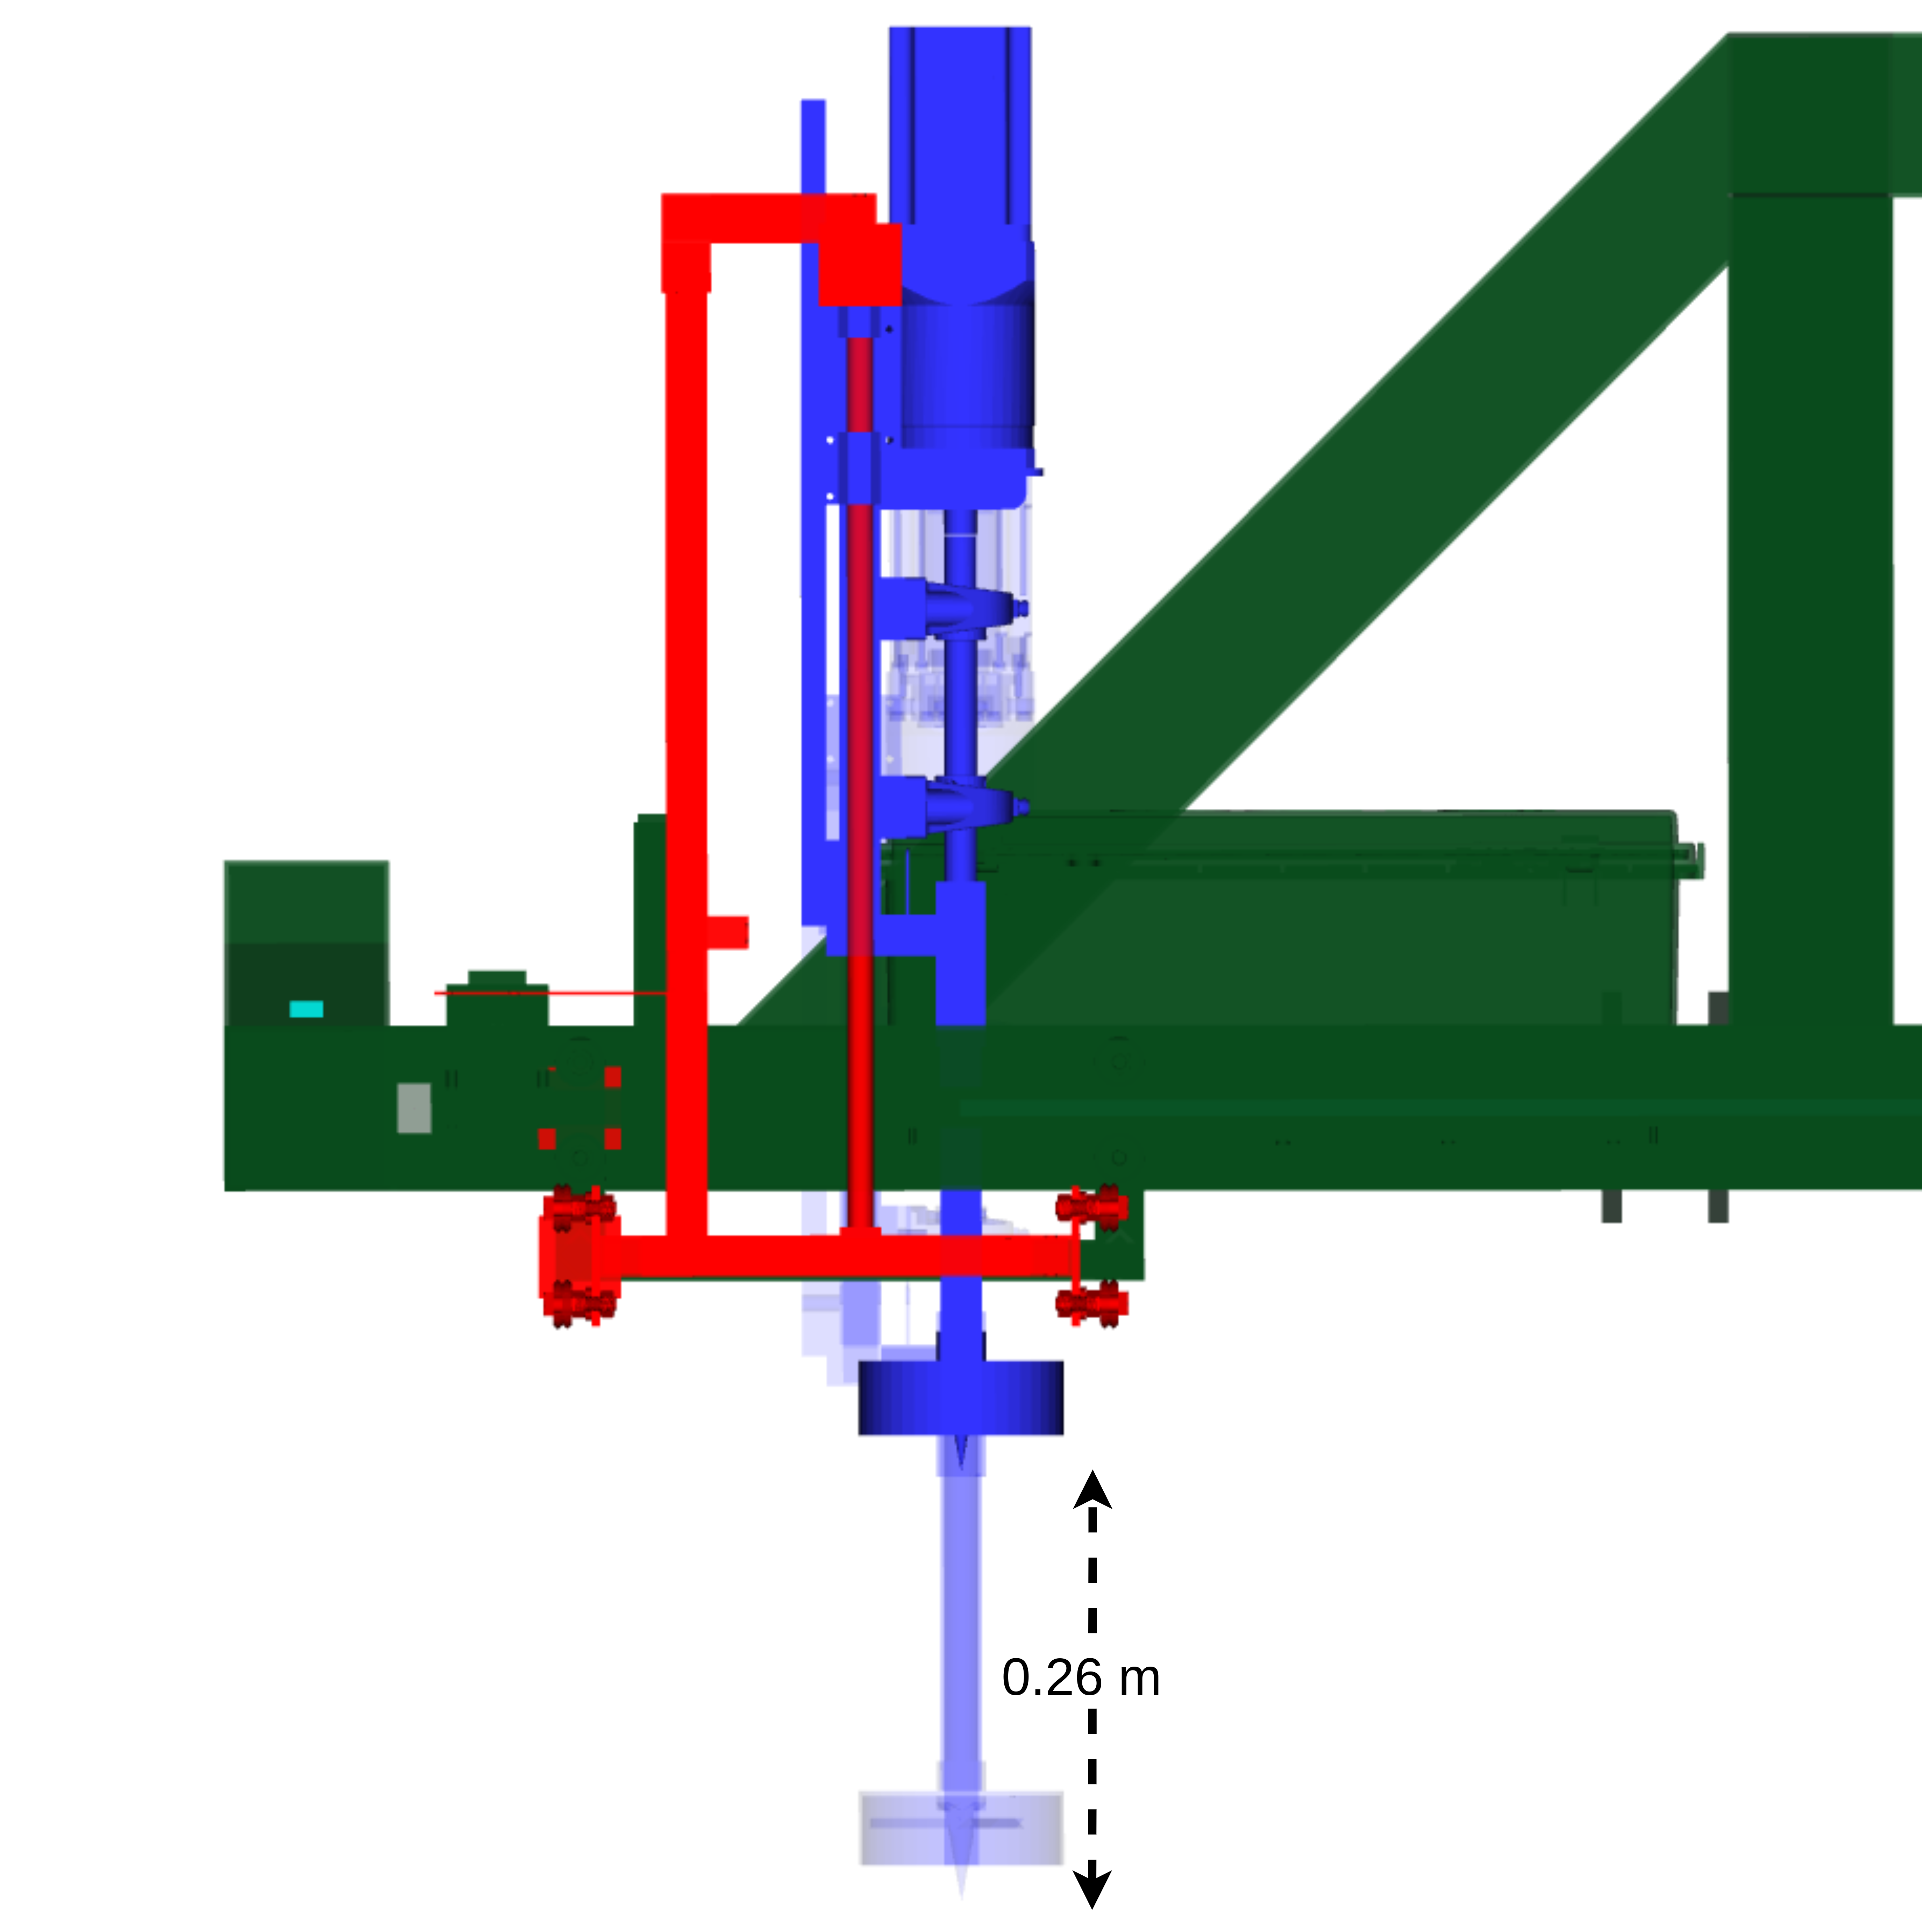
\includegraphics[width=.45\linewidth]{gfx/ch02/z_ws.png}} \\
    \caption{\ac{IT} Workspace Layout}\label{fig:ws}
\end{figure}

The \ac{IT} is controlled using ROS$2$ actions, which provide a structured way to handle asynchronous tasks with feedback and result reporting. For the $XY$ movement of the gantry, the \texttt{AxisPosition} action is used, allowing the specification of target coordinates ($x$, $y$) and speed, while providing feedback on the current position and confirming whether the target was reached. The \texttt{Extraction} action manages the vertical movement of the tool along the $Z$ axis, reporting the depth reached, total time taken, and success status, along with real-time feedback on the current depth. Finally, the \texttt{ExtractionCycle} action coordinates the execution of multiple extractions by accepting an array of target poses and their corresponding IDs, providing feedback on the current status and reporting the results of the extraction process for each pose. These actions enable precise and modular control of the gantry system, ensuring efficient and reliable operation. A diagram summarizing this process is shown in \autoref{fig:gantry-control}.

\begin{figure}[h]
    \centering
    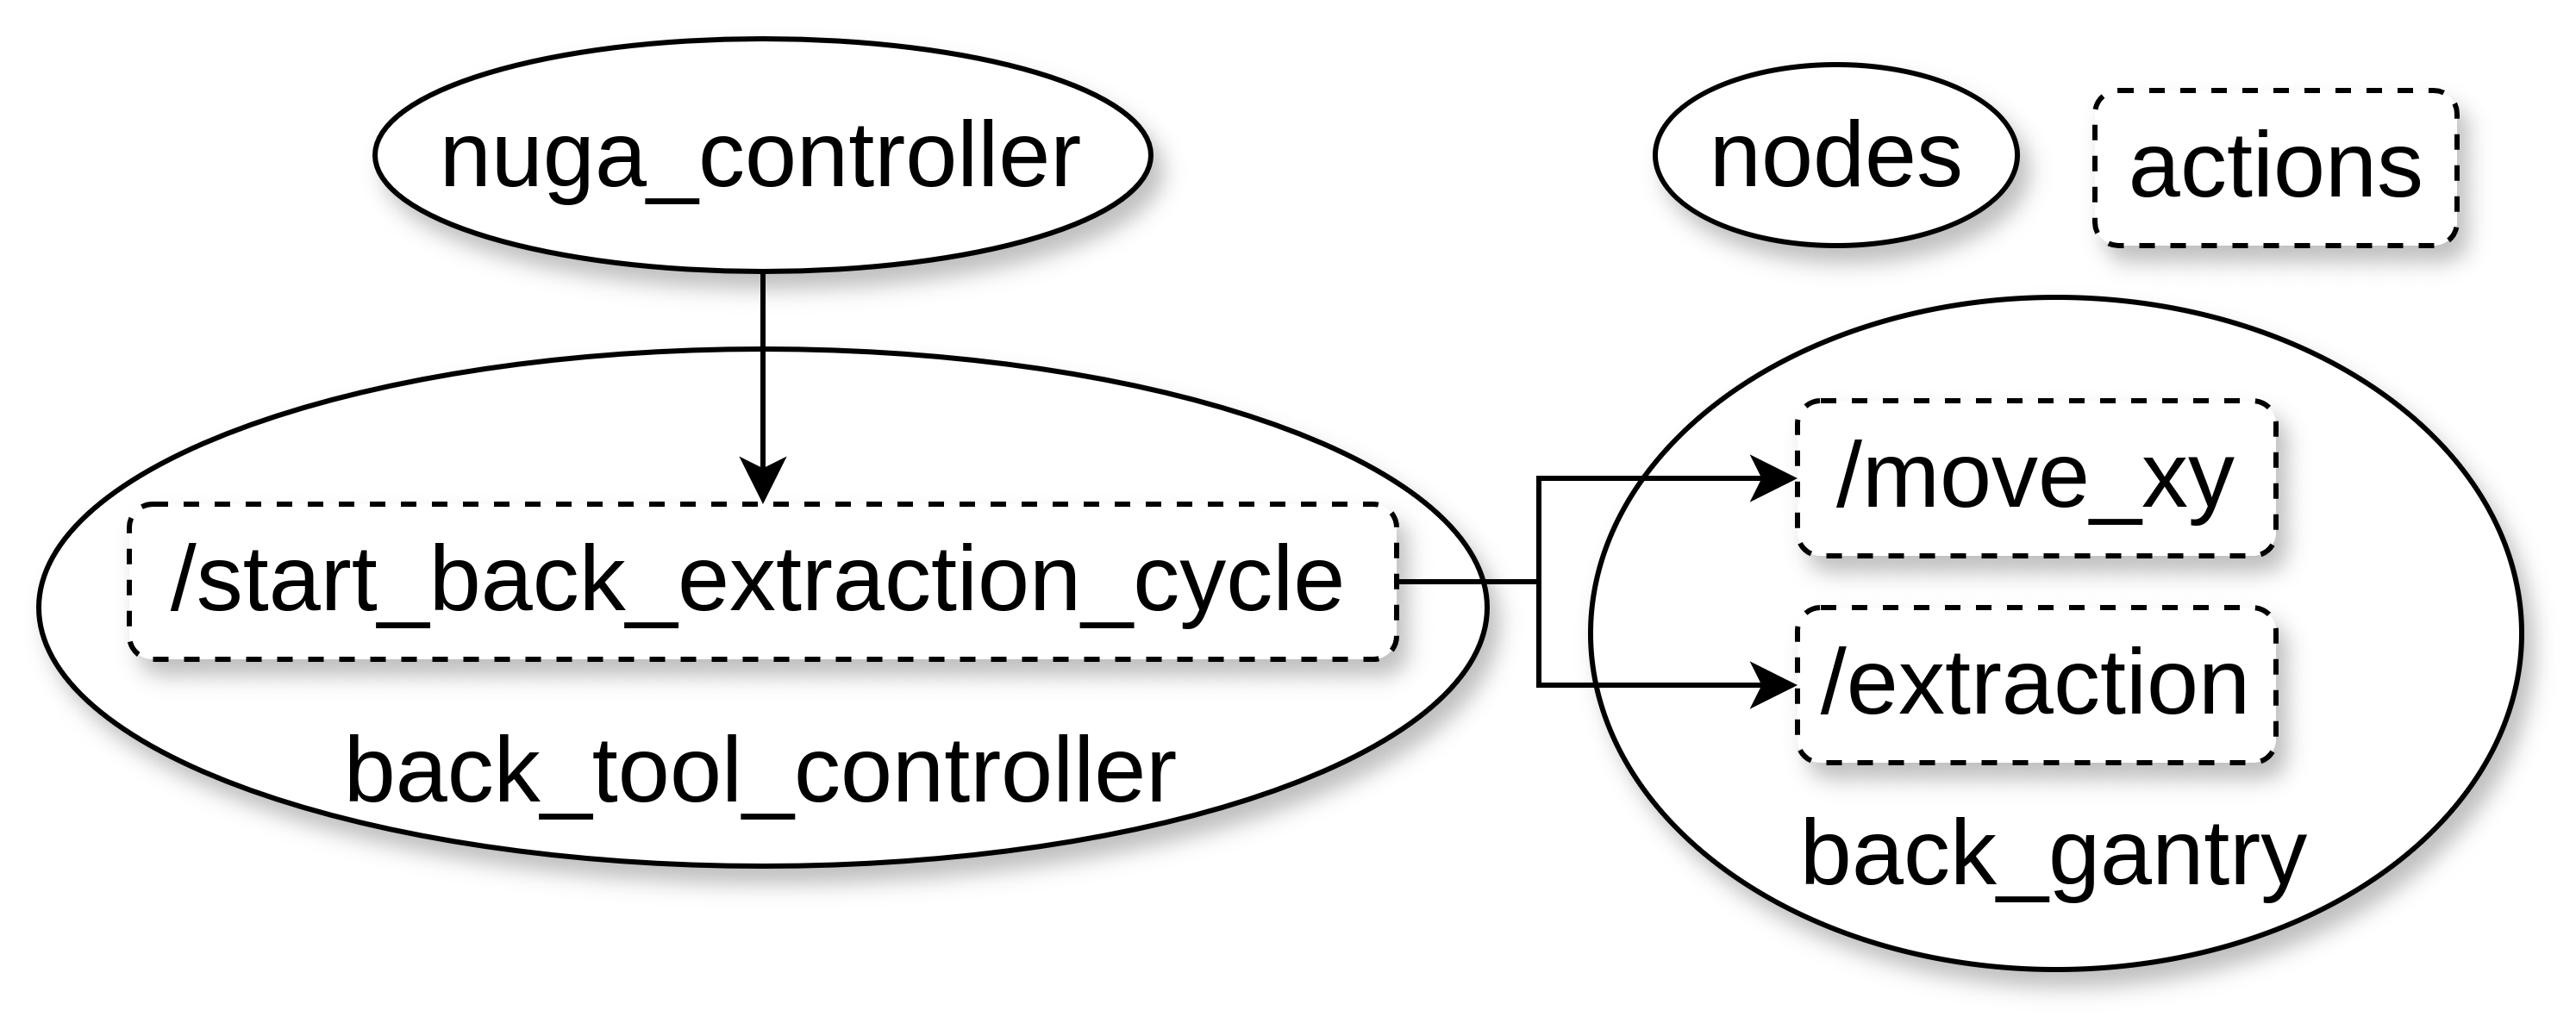
\includegraphics[width=0.7\linewidth]{gfx/ch02/gantry_control.png}
    \caption{ROS Interface for back gantry control}
    \label{fig:gantry-control}
\end{figure}


\subsection{Localization}
\lipsum[1]

\subsection{Weed Detection}
\lipsum[1]


%*****************************************
%*****************************************
%*****************************************
%*****************************************
%*****************************************
